\documentclass[11pt,a4paper]{article}

\usepackage{polski}
\usepackage[polish]{babel}
%\usepackage[none]{hyphenat} %no hyphen breaks
\usepackage[utf8]{inputenc}

%font
\usepackage[sfdefault]{roboto} %% option 'sfdefault' activates Sans as the default text font
\usepackage[T1]{fontenc}

\usepackage{color}

\usepackage{graphicx}

\usepackage{pdfpages}

%justify - no hyphens
\tolerance=1000
\emergencystretch=\maxdimen
\hyphenpenalty=1000
\hbadness=10000

%colors
\definecolor{darkyellow}{RGB}{244,213,9}
\definecolor{darkgreen}{RGB}{28,135,12}

\usepackage{enumitem}
%\setenumerate[1]{leftmargin=2.9cm,label=\Alph*.}
\setenumerate[1]{leftmargin=1.2cm,label=\textcolor{darkgreen}{\Alph*.}}
\setenumerate[2]{label=\textbf{\roman*.}}
\setenumerate[3]{label=\textbf{\alph*.}}
\setenumerate[4]{label=\textbf{\arabic*.}}

% Section numbering
\setcounter{secnumdepth}{5}
\setcounter{tocdepth}{2}

\usepackage{letltxmacro}

% Unnumbered sections included in ToC
\newcommand{\psection}[1]{
  \section*{#1}
  \addcontentsline{toc}{section}{#1}
}
\newcommand{\psubsection}[1]{
  \subsection*{#1}
  \addcontentsline{toc}{subsection}{#1}
}

\usepackage[explicit]{titlesec}
\usepackage{ulem}
\titleformat{\section}{\normalfont\Large\bfseries}{\thesection.}{2ex}{#1}
\titleformat{\subsection}{\normalfont\large\bfseries}{\thesubsection.}{1.5ex}{#1}
\titleformat{\subsubsection}{\normalfont\normalsize\bfseries}{\thesubsubsection.}{1ex}{#1}
\titleformat{\paragraph}[block]{\normalfont\normalsize}{}{0pt}{\uline{\theparagraph.\hspace*{1ex}#1}} %

%custom spacing
% \titlespacing*{\subsection}{0.5cm}{0pt}{0pt}
%\titlespacing*{\subsubsection}{1.3cm}{0pt}{0pt}
%\titlespacing*{\paragraph}{2cm}{0pt}{0pt}

% Indent subsubsections
\newenvironment{indentpar}[1]%
  {\begin{list}{}%
          {\setlength{\leftmargin}{#1}}%
          \item[]%
  }
  {\end{list}}


% \LetLtxMacro{\oldsubsection}{\subsection}
% \renewcommand{\subsection}[1]{
%   \oldsubsection{#1}%
%   \leftskip0.5cm
% }
% \LetLtxMacro{\oldsubsubsection}{\subsubsection}
% \renewcommand{\subsubsection}[1]{
%   \oldsubsubsection{#1}%
%   \leftskip1.3cm
% }
% \LetLtxMacro{\oldparagraph}{\paragraph}
% \renewcommand{\paragraph}[1]{
%   \oldparagraph{#1}%
%   \leftskip2cm
% }

% Custom subparagraphs
\newcommand\redcard[1]{\bgroup\textcolor{darkgreen}{\textbf{Kara: }}\bgroup\textcolor{red}{\textbf{Czerwona Kartka}} -- #1}
\newcommand\yellowcard[1]{\bgroup\textcolor{darkgreen}{\textbf{Kara: }}\bgroup\textcolor{darkyellow}{\textbf{Żółta Kartka}} -- #1}
\newcommand\bluecard[1]{\bgroup\textcolor{darkgreen}{\textbf{Kara: }}\bgroup\textcolor{blue}{\textbf{Niebieska Kartka}} -- #1}
\newcommand\penaltyd[2]{\bgroup\textcolor{darkgreen}{\textbf{Kara: #1}} -- #2}

\usepackage{geometry}

\newcommand\image[2]{
	\newgeometry{left=0cm,top=#2}
	\includegraphics[width=\paperwidth]{#1}
	\restoregeometry
}

\setlength{\parindent}{0pt} % brak wcięć
\setlength{\parskip}{1ex plus 0.5ex minus 0.2ex}
\normalem %emphasis isn't underline
\linespread{1.1} %interlinia

\title{Zasady gry w~quidditcha}
\author{Polska Liga Quidditcha}
\date{Sezon 2018 - 2019}

\begin{document}

\maketitle

\setlength{\parskip}{0ex}

\tableofcontents

\setlength{\parskip}{1ex plus 0.5ex minus 0.2ex}

\newpage

\psection{Wstęp}

Popularność quidditcha stale rośnie i~rozwija się on w~dynamiczną i~ambitną dyscyplinę sportową,
wymagającą nie lada wysiłku fizycznego,
złożonych strategii i~nielichych umiejętności.

Każdego dnia treningi i mecze quidditcha odbywają się w 40 krajach na całym świecie.
W ciągu ostatnich dwóch lat ten sport przeżył niesamowity skok w rozwoju, co oznacza,
że zasady również muszą być rozwijane. Bazując na opiniach graczy, sędziów i trenerów
dokonaliśmy odpowiednich modyfikacji, mających polepszyć przyszłość quidditcha.

Rulebook został skondensowany, część zasad lepiej wyjaśniona, a niektóre elementy gry
zmienione. Mamy nadzieję, że te zmiany pomogą ustalić poprawny kierunek dla sportu, aby gracze
z całego świata byli podekscytowani quidditchem.

To wydanie \emph{Zasad gry w~quidditcha} opiera się na Rulebooku 2018-2020 wydanym przez IQA.

Polska Liga Quidditcha dziękuje wszystkim zaangażowanym (w kolejności alfabetycznej) w stworzenie przekładu niniejszych \emph{Zasad} z języka angielskiego:
\begin{center}
	\begin{tabular}{c c}

	\end{tabular}
\end{center}

%\image{team_poland}{6cm}
\pagebreak

\section{Drużyna i ławka rezerwowych}

\subsection{Kapitan oraz personel drużyny}

\subsubsection{Obowiązkowy \emph{speaking captain}}
Każda drużyna musi wyznaczyć jedną osobę, która będzie
wpisana w oficjalny roster, aby pełniła rolę
\emph{speaking captain} podczas gry.

\begin{enumerate}
  \item \emph{Speaking captain} może rozmawiać z
  \emph{officials} w imieniu całej drużyny.
  \begin{enumerate}
    \item Zawodnicy mogą rozmawiać z \emph{officials} w
    swojej sprawie.
    \item \emph{Officials} mogą nakazać dowolnej osobie
    zaprzestania mówienia do dowolnego \emph{official}.
  \end{enumerate}

  \item Jeśli wyznaczony \emph{speaking captain} nie jest w
  stanie kontynuować swoich obowiązków, z dowolnego względu,
  drużyna musi wybrać jego zastępcę.
  \begin{enumerate}
    \item Jeśli poprzedni \emph{speaking captain} legalnie
    powróci na boisko lub ławkę rezerwowych, na powrót
    przejmuje obowiązki \emph{speaking captain}.
  \end{enumerate}

  \item \emph{Speaking captain} nie może wejść na boisko,
  jeśli gra nie została zatrzymana, chyba że wchodzi jako 
  gracz.
  \begin{enumerate}
    \item Jeśli \emph{speaking captain} znacząco wejdzie na
    boisko lub wpłynie na grę w jakikolwiek sposób będąc
    nielegalnie na boisku, liczy się to jako wtargnięcie na
    boisko.
  \end{enumerate}
\end{enumerate}

\bluecard{Wtargnięcie na boisko.}

\subsubsection{Personel drużyny}
Niegrający członkowie drużyny, włączając niegrających
coachów, to personel drużyny.
\begin{enumerate}
  \item Organizatorzy turnieju mogą ograniczyć liczbę
  członków personelu drużyny, którzy mogą przebywać
  wewnątrz strefy graczy.
  \begin{enumerate}
    \item Ograniczenie musi pozwolić na conajmniej trzech
    członków personelu drużyny.
  \end{enumerate}

  \item Personel drużyny nie może wejść do gry.
  \item Jeśli członek personelu drużyny zrobi coś co
  skutkowałoby karą dla zawodnika rezerwowego, to ten
  członek personelu musi dostać tą samą karę.
  \item Personel drużyny nie może wchodzić na boisko jeśli
  gra nie jest zatrzymana.
  \begin{enumerate}
    \item Jeśli członek personelu drużyny znacząco wejdzie
    na boisko lub wpłynie na grę w jakikolwiek sposób będąc
    nielegalnie na boisku, liczy się to jako wtargnięcie
    na boisko.
  \end{enumerate}
\end{enumerate}

\bluecard{Wtargnięcie na boisko.}

\subsection{Roster i zawodnicy}

\subsubsection{Roster}
\begin{enumerate}
  \item Drużyna składa się z minimum siedmiu i maksymalnie
  21 zawodników.
  \begin{enumerate}
    \item Drużyna musi mieć siedmiu zdolnych do gry zawodników, aby rozpocząć lub kontynuować grę.
    \begin{enumerate}
      \item Jeśli drużyna nie będzia miała conajmniej siedmiu zdolnych do gry zawodników w dowolnym momencie gry, taka drużyna musi się poddać.
    \end{enumerate}
  \end{enumerate}
\end{enumerate}

\penaltyd{Poddanie się}{Drużyna nie posiada 7 zawodników zdolnych do gry.}

\subsubsection{Pozycje}
\begin{enumerate}
  \item Drużyna ma jednego obrońcę w grze.
  \begin{enumerate}
    \item Obrońcy muszą nosić zieloną opaskę na czole.
    \item Obrońcy mogą używać kafla na każdy legalny sposób.
  \end{enumerate}

  \item Drużyna ma trzech ścigających w grze.
  \begin{enumerate}
    \item Ścigający muszą nosić białą opaskę na czole.
    \item Ścigający mogą używać kafla na każdy legalny sposób.
  \end{enumerate}

  \item Drużyna ma dwóch pałkarzy w grze.
  \begin{enumerate}
    \item Pałkarze muszą nosić czarną opaskę na czole.
    \item Pałkarze mogą używać tłuczków na każdy legalny sposób.
  \end{enumerate}

  \item Podczas \emph{seeker floor}, drużyna nie może mieć w grze szukającego. Po za nim, drużyna musi mieć szukającego w grze.
  \begin{enumerate}
    \item Szukający muszą nosić żółtą opaskę na czole.
  \end{enumerate}

  \item Zawodnicy poza grą są zawodnikami rezerwowymi.
  \begin{enumerate}
    \item Zawodnicy rezerwowi nie mają przypisanej pozycji.
    \item Zawodnicy rezerwowi nie muszą mieć na głowie żadnej opaski.
  \end{enumerate}

  \item Zawodnicy w \emph{penalty box} uznawani są jako w grze i liczą się do wymogów pozycji dla swojej drużyny.

  \item Nie można ukarać drużyny za chwilowe niespełnienie wymogów pozycji ze względu na zmianę zawodników lub jeśli szukający zagapi się i nie wejdzie na boisko po zakończeniu \emph{seeker floor}.

\end{enumerate}

\yellowcard{(\emph{Speaking captain}) Nieprzestrzeganie wymogów pozycji w grze.}

\yellowcard{(\emph{Speaking captain}) Umyślne niewystawienie szukającego do gry.}

\subsubsection{Zasada gender}
\begin{enumerate}
  \item Drużyna może mieć conajwyżej czterech zawodników identyfikujących się z daną płcią w grze, w tym samym czasie.
  \begin{enumerate}
    \item Zawodnik przebywający w \emph{penalty box} uznawany jest jako w grze.
  \end{enumerate}

  \item Płeć z jaką zawodnik się identyfikuje uznawana jest za płeć tego zawodnika.

  \item Jeśli drużyna nie może wystawić pełnego zestawu zawodników, bo nie spełniłaby zasady gender, to może kontynuować grę z mniejszą ilością zawodników na boisku.
  \begin{enumerate}
    \item Drużyna nie może rozpocząć gry, jeśli nie spełniają wymogów pełnego zestawu zawodników.
    \item Jeden obrońca, jeden pałkarz i jeden ścigający są obowiązkowo w grze, nawet jeśli drużyna wystawia mniej niż siedmiu zawodników.
    \begin{enumerate}
      \item Wliczamy w to zawodników w \emph{penalty box}.
      \item Po zakończeniu \emph{seeker floor}, jeden szukający również jest obowiązkowy.
    \end{enumerate}
    \item Jeśli drużyna odzyska możliwość wystawienia pełnego zestawu zawodników to musi to zrobić.
    \begin{enumerate}
      \item W tym przypadku zawodnik wchodzi na boisko z ławki rezerwowych.
    \end{enumerate}
  \end{enumerate}
\end{enumerate}

\yellowcard{(\emph{Speaking captain}) Nieprzestrzeganie wymogów zestawu zawodników w grze.}

\subsubsection{Poprawianie niewłaściwego zestawu zawodników}
Kiedy \emph{speaking captain} otrzyma karę za nieprzestrzeganie wymogów zestawu zawodników w grze, drużyna musi naprawić sytuację jak najmniejszą liczbą zmian zanim gra zostanie wznowiona.

\subsection{Zmiany}

\subsubsection{Procedura zmiany}
Aby wymienić zawodnika z rezerwowym kiedy gra nie jest wstrzymana muszą nastąpić poniższe:
\begin{enumerate}
  \item Zawodnik schodzący z boiska nie jest zbity.
  \item Zawodnik schodzi z boiska w strefie zmian swojej drużyny, a następnie schodzi z miotły.
  \begin{enumerate}
    \item Zawodnik nie może zejść z miotły zanim opuści boisko.
    \item Zawodnik, który zszedł z miotły aby się zmienić, nie może już być zbity.
  \end{enumerate}
  \item Wszelkiego rodzaju wymiana sprzętu (również opasek) musi się odbyć poza boiskiem.
  \item Zawodnik rezerwowy wchodzący do gry wsiada na miotłę w strefie zmian i wchodzi na boisko zanim będzie mógł wejść w interakcję z grą.
  \begin{enumerate}
    \item Zawodnik rezerwowy wchodzi na boisko mniej więcej w tym samym miejscu, gdzie zmieniający się zawodnik z niego zszedł.
    \item Zmiana jest zakończona gdy zawodnik przekroczy krawędź boiska i dotyka tylko ziemię na boisku.
    \begin{enumerate}
      \item W tym momencie zawodnik może zacząć interakcje z grą i może zostać zbity.
    \end{enumerate}
  \end{enumerate}
  \item Wchodzący na boisko zawodnik dostaję karę jeśli niewłaściwie przeprowadzono zmianę.
  \item Jeśli zawodnik wejdzie na boisko po niewłaściwym przeprowadzeniu zmiany, ale jeszcze nie wejdzie w interakcję z grą, \emph{official} powinien nakazać mu powtórzenie procedury.
  \begin{enumerate}
    \item Jeśli zawodnik wejdzie w interakcję z grą przed decyzją \emph{official} lub przed poprawieniem procedury, musi być ukarany za nielegalną zmianę.
    \item Zawodnik, który wielokrotnie nieprzestrzega procedury zmiany, musi być ukarany za nielegalną zmianę.
  \end{enumerate}
\end{enumerate}

\penaltyd{Powtórz procedurę}{Niewłaściwe przeprowadzenie zmiany.}

\bluecard{Nielegalna zmiana.}

\subsubsection{Zmiana pozycji}
Zawodnicy mogą wymienić się pozycjami przez przeprowadzenie procedury zmiany i wymianę opasek, po tym jak zeszli z mioteł w strefie zmian.
\begin{enumerate}
  \item Kiedy zawodnicy się wymieniają opaski to obserwujemy dwie oddzielne zmiany. Schodzą z boiska jako zawodnik starej pozycji i wchodzą jako zawodnik nowej pozycji.
\end{enumerate}

\subsubsection{Zasady zmian}
\begin{enumerate}
  \item Zmiany mogą być przeprowadzane tylko kiedy gra nie jest wstrzymana, z poniższymi wyjątkami:
  \begin{enumerate}
    \item Zmiana zawodnika wyrzuconego z boiska (patrz 9.1.6. Wyrzucenie) %TODO ref
    \item Zmiana zawodnika kontuzjowanego (patrz 1.3.4. Zmiana z powodu kontuzji) %TODO ref
    \item Obrońca zamienia się pozycją z innym zawodnikiem kiedy idzie do \emph{penalty box} (patrz 9.4.2.) %TODO ref
    \item Zamiana zawodnika z rezerwowym, który popełnił faul (patrz 9.4.5.) %TODO ref
    \item Poprawianie niewłaściwego zestawu zawodników po otrzymaniu kary (patrz 1.2.4.) %TODO ref
  \end{enumerate}
\end{enumerate}

\subsubsection{Zmiana z powodu kontuzji}
\begin{enumerate}
  \item Jeśli zawodnik dozna kontuzji ale gra nie została wstrzymana, to aby się zmienić musi przejść procedurę zmiany (patrz 1.3.1.) %TODO ref
  \item Gra musi zostać wstrzymana jeśli zawodnik krwawi lub leży i jest zbyt mocno kontuzjowany aby kontynuować grę lub się zmienić.
  \begin{enumerate}
    \item Gra powinna zostać wstrzymana natychmiast jeśli kontuzjowany zawodnik znajduje się w pobliżu akcji lub został poważnie kontuzjowany, włączając w to niepowierzchowne urazy głowy.
    \item Jeśli kontuzja nie jest poważna, a zawodnik nie przeszkadza w dalszym rozegraniu akcji, sędzia główny powinien pozwolić grze na kontynuację, dopóki jej zatrzymanie nie będzie powodowało przewagi dla którejś z drużyn lub gra zbliży się do kontuzjowanego zawodnika.
  \end{enumerate}
  \item Jeśli gra została wstrzymana i zawodnik jest kontuzjowany:
  \begin{enumerate}
    \item Kontuzjowany zawodnik może opuścić boisko i zostać zastąpionym przez zawodnika rezerwowego.
    \begin{enumerate}
      \item Jeśli gra została wstrzymana z powodu kontuzji zawodnika, to musi on opuścić boisko.
      \item Jeśli zawodnik krwawi, musi opuścić boisko.
      \begin{enumerate}
        \item Krwawiący zawodnik nie może powrócić do gry, dopóki nie otrzyma pozwolenia od \emph{official}, który uzna, że krwawienie ustało.
      \end{enumerate}
      \item Miotła kontuzjowanego zawodnika pozostaje na boisku tam gdzie była gdy gra została wstrzymana.
    \end{enumerate}
    \item Kontuzjowany zawodnik, który opuszcza boisko musi być zastąpiony dowolnym rezerwowym nadającym się do gry.
    \begin{enumerate}
      \item Podczas wstrzymania gry, rezerwowy zamienia zawodnika w miejscu oznaczonym przez jego miotłę.
      \item Jeśli nie ma żadnych nadających się rezerwowych, spełniających zasadę gender, drużyna może grać z jednym zawodnikiem mniej.
      \begin{enumerate}
        \item Jeśli to by oznaczało brak zawodnika o danej pozycji, to inny zawodnik musi zająć pozycję i miejsce na boisku kontuzjowanego zawodnika.
      \end{enumerate}
      \item Jeśli zawodnik jest zmuszony przez zasady do opuszczenia boiska, ale ma lekką kontuzję i może grać dalej, a nie ma stosownych rezerwowych, to zawodnik ten może wziąć miotłę i kontynuować grę od granicy strefy zmian.
    \end{enumerate}
  \end{enumerate}
  \item Zawodnik nie może symulować kontuzji.
\end{enumerate}

\yellowcard{Symulowanie kontuzji.}

\subsubsection{Zmiany między etapami gry}
Drużyny mogą robić dowolnie wiele zmian między etapami gry nie wykonując procedury zmiany.
\begin{enumerate}
  \item Zawodnik przebywający w \emph{penalty box} nie może zostać zmieniony między etapami gry.
  \item Jeśli zawodnik otrzyma kartkę za faul popełniony po tym jak sędzia główny oznajmił koniec etapu gry, ta kara powinna zostać potraktowana jako kara dla zawodnika rezerwowego, a \emph{speaking captain} może wybrać pozycję, pod którą faulujący zawodnik odbędzie karę.
\end{enumerate}

\yellowcard{(\emph{Speaking captain}) Nielegalna zmiana między etapami gry.}

\subsection{Strefa zmian i ławka drużyny}

\subsubsection{Ograniczenia ławki drużyny i strefy zmian}
\begin{enumerate}
  \item Wszelkie zmiany muszą odbyć się w strefie zmian, a nie w ławce drużyny.
  \item Zawodnicy rezerwowi i personel drużyny muszą przebywać na ławce drużyny lub strefie zmian kiedy gra nie jest wstrzymana i nie mogą tłumić się przy granicy boiska o ile nie będą za chwilę się zmieniać.
  \begin{enumerate}
    \item Jeśli drużyna wielokrotnie tłumi się przy granicy boiska, \emph{officials} mogą nakazać rezerwowym pozostanie tylko na ławce drużyny, o ile zaraz taki zawodnik nie będzie się zmieniał.
  \end{enumerate}
  \item Wszelkiego rodzaju sprzęt, który nie jest niezbędny do gry, musi pozostać na ławce drużyny.
  \begin{enumerate}
    \item Wszelkie dodatkowe piłki drużyny mogą znajdować się na ławce, ale muszą być schowane w torbie lub innym pojemniku.
  \end{enumerate}
\end{enumerate}

\subsubsection{Opuszczanie strefy zmian, ławki lub strefy graczy}
\begin{enumerate}
  \item Jeden zawodnik rezerwowy lub członek personelu drużyny może opuścić strefę zmian lub ławkę drużyny, aby sprawdzić czas lub wynik, ale nie może przeszkadzać \emph{timekeeper} i \emph{scorekeeper} w ich obowiązkach, ani wejść na boisko.
  \item \emph{Speaking captain} może opuścić strefę graczy, aby porozumieć się z organizatorami turnieju.
  \item Każdy kto potrzebuje pomocy medyków może opuścić strefę graczy, aby ją otrzymać.
  \begin{enumerate}
    \item Każdy zawodnik, który opuści w ten sposób strefę graczy, może wrócić do gry jeśli medycy uznają, że może.
    \item Jeśli zajdzie taka potrzeba, to \emph{speaking captain} może wyznaczyć osobę, która opuści strefę graczy, aby pomóc kontuzjowanemu zawodnikowi.
    \item W przypadku urazu głowy zawodnika, sędzia główny może nakazać mu opuszczenie strefy gry, aby zasięgnąć pomocy medyków.
  \end{enumerate}
  \item Celowe nielegalne opuszczenie strefy zmian lub ławki drużyny, mające na celu obejście zasad to nielegalne obejście.
\end{enumerate}

\bluecard{Nielegalne obejście.}

\subsubsection{Przeszkadzanie przy liniach bocznych}
Zawodnicy rezerwowi nie mogą przeszkadzać grze przy liniach bocznych.
\begin{enumerate}
  \item Rezerwowy przeszkadza przy linii bocznej jeśli bezpośrednio oddziaływuje na grę i zachodzi jedno z poniższych:
  \begin{enumerate}
    \item Rezerwowy jest nielegalnie i celowo poza strefą zmian i ławką drużyny.
    \item Rezerwowy nie usiłował odsunąć się, aby uniknąć interakcji z grą.
  \end{enumerate}
\end{enumerate}

\bluecard{Przeszkadzanie przy liniach bocznych}

\redcard{Celowe przeszkadzanie przy liniach bocznych}

\section{Sprzęt i wymiary boiska}
%TODO img

\subsection{Linie i oznaczenia boiska}

\subsubsection{Linie granic}
Boisko składa się z czterech granic, które tworzą prostokąt 33m na 60m.
\begin{enumerate}
  \item Linie granic długości 33m to linie końcowe.
  \item Linie granic długości 60m to linie boczne.
  \begin{enumerate}
    \item Linia boczna najbliższej stołu \emph{scorekeeper} to linia boczna \emph{scorekeepera}.
  \end{enumerate}
\end{enumerate}

\subsubsection{Linia środkowa}
Linia środkowa łączy środki linii bocznych.

\subsubsection{Linie pola obrońcy}
Są dwie linie pola pola obrońcy, równoległe do linii końcowych, łączące linie boczne i usytuowane są 11 metrów od linii środkowej, bo obu jej stronach.

\subsubsection{Linie bramkowe}
Są dwie linie bramkowe, równoległe do linii końcowych, łączące linie boczne i usytuowane są 16,5 metra od linii środkowej, bo obu jej stronach.

%TODO img
\subsubsection{\emph{Penalty boxes}}
Każda drużyna ma \emph{penalty box} poza boiskiem.
\begin{enumerate}
  \item Każdy \emph{penalty box} to kwadrat o boku 5,5 metra, zaczynający się na linii środkowej i ciągnący w stronę ławki drużyny przy linii bocznej \emph{scorekeepera}.
\end{enumerate}

\subsubsection{Pozycje piłek}
Na linii środkowej są oznaczone cztery pozycje piłek.
\begin{enumerate}
  \item Pierwsze dwie piłki są położone 2,75m po obu stronach linii środkowej.
  \item Kolejne dwie piłki są położone 8,25m po obu stronach linii środkowej.
\end{enumerate}

\subsubsection{Strefy zmian}
Strefa zmian to prostokąt 19m na 2,75m poza boiskiem graniczący z polem obrońcy drużyny po stronie linii bocznej \emph{scorekeppera}.

\subsubsection{Ławki drużyn}
Ławka drużyny to prostokąt 19m na 2,75m przylegający dłuższym bokiem do strefy zmian drużyny i dotykający granicy strefy gracza.

%TODO img

\subsubsection{Strefa graczy}
Strefa graczy to prostokąt, który po środku ma boisko.
\begin{enumerate}
  \item Prostokąt ten ma wymiary 44m na 66m.
  \item Strefa graczy nie może zawierać żadnych przeszkód ani niebezpiecznego terenu.
  \begin{enumerate}
    \item Żadne elementy turniejowe, np. stół \emph{scorekeeper}, nie mogą być ustawione wewnątrz strefy graczy.
  \end{enumerate}
  \item Podczas gry strefa graczy jest zarezerwowana dla:
  \begin{enumerate}
    \item Zawodników w grze.
    \item Sędziów i \emph{officials} przypisanych do danej gry.
    \item Organizatorów turnieju, którzy otrzymali uprawnienia (na swoje ryzyko) od sędziego głównego lub dyrektora turnieju.
    \item Personel drużyny zgodnie z opisem w 1.1.2 %TODO ref
  \end{enumerate}
  \item Widzowie nie mogą wchodzić do strefy graczy.
\end{enumerate}

%TODO img

\subsubsection{Oznaczenia boiska}
Poszczególne części boiska i otaczającej strefy powinny być oznaczone w jasny sposób. Te oznaczenia zazwyczaj robi się rysując linie lub stawiając znaczniki stożkowe.
\begin{enumerate}
  \item Poniższe muszą być oznaczone:
  \begin{enumerate}
    \item Granice boiska (2.1.1.) %TODO ref
    \item Linia środkowa (2.1.2.) %TODO ref
    \item Linie pola obrońcy (2.1.3.) %TODO ref
    \item Pozycja piłki najbardziej oddalona od stołu \emph{scorekeepera} (2.1.6.) %TODO ref
  \end{enumerate}
  \item Poniższe oznaczenia są opcjonalne, ale zalecane:
  \begin{enumerate}
    \item Linie bramkowe (2.1.4.) %TODO ref
    \item \emph{Penalty boxes} (2.1.5.) %TODO ref
    \item Pozostałe pozycje piłek (2.1.6.) %TODO ref
    \item Ławki drużyn (2.1.8.) %TODO ref
    \item Strefa graczy (2.1.9.) %TODO ref
    \item Pozycje pętli (2.2.3.) %TODO ref
    \begin{enumerate}
      \item Te oznaczenia nie mogą wpływać na stabilność pętli.
    \end{enumerate}
  \end{enumerate}
\end{enumerate}

%TODO img

\subsection{Pętle}

\subsubsection{Konstrukcja pętli}
\begin{enumerate}
  \item Każda pętla musi się składać ze słupa i okgrągłej obręczy na szczycie słupa. Materiał ich wykonania może być dowolny, poza metalem i cementem, i nie może stanowić zagrożenia dla graczy.
  \item Pętla może być umieszczona na podstawce, aby stała pionowo.
  \begin{enumerate}
    \item Wielkość podstawki nie może naruszać wysokości pętli.
    \item Podstawka może zawierać metalowe mocowania, ale nie może być wykonana z metalu lub cementu.
  \end{enumerate}
  \item Pętle muszą samodzielnie stać i wytrzymać grę.
  \begin{enumerate}
    \item Sędziowie muszą odmówić gry na pętlach lub podstawkach, które ich zdaniem są niebezpieczne dla graczy.
  \end{enumerate}
\end{enumerate}

\subsubsection{Kształt pętli}
\begin{enumerate}
  \item Każdy zestaw pętli ma trzy słupy o różnych wysokościach.
  \begin{enumerate}
    \item Te wysokości to 0,91m, 1,37m, 1,83m.
  \end{enumerate}
  \item Obręcz musi być zamocowana do szczytu każdego słupa.
  \begin{enumerate}
    \item Wewnętrzna średnica obręczy musi wynosić między 81cm, a 86cm.
    \item Mocowanie obręczy do słupa nie może spowodować, że słup będzie wyższy niż jego wymagana wysokość.
  \end{enumerate}
\end{enumerate}

\subsubsection{Pozycje pętli}
\begin{enumerate}
  \item Trzy pętle są umieszczone na linii bramkowej.
  \begin{enumerate}
    \item Najwyższa pętla (1,83cm) musi być umieszczona na środku linii bramkowej.
    \item Pozostałe dwie pętle umieszczane są na linii bramkowej w odległości 234cm po obu stronach najwyższej pętli.
    \item Patrząc na pętle ze środka boiska, mała pętla (0,91m) musi być po lewej stronie, a średnia (1,37m) po prawej stronie.
  \end{enumerate}
  \item Obręcze pętli muszą być obrócone tak aby ich płaszczyzna zawierała linię bramkową.
\end{enumerate}

\subsection{Piłki}

\subsubsection{Kafel}
Kafel musi spełniać poniższe:
\begin{enumerate}
  \item Być piłką do siatkówki.
  \item Mieć między 65cm a 67cm w średnicy.
  \item Kafel musi zachowywać okrągły kształt, nie może być w pełni napompowany, ani tak spompowany, aby zawodnik był w stanie złapać wałek pokrycia jedną ręką.
\end{enumerate}

\subsubsection{Tłuczki}
Trzy tłuczki muszą spełniać:
\begin{enumerate}
  \item Być okrągłą piłką zrobioną z elastycznego, gumowego lub podobnego tworzywa (np. dodgeball).
  \item Mieć 22cm w średnicy i 68cm w obwodzie.
  \item Tłuczki muszą zachowywać okrągły kształt, nie mogą być w pełni napompowane, ani tak spompowane, aby zawodnik był w stanie złapać wałek pokrycia jedną ręką.
\end{enumerate}

\subsubsection{Ogonek zniczowy}
Ogonek zniczowy powinien spełniać:
\begin{enumerate}
  \item Być piłką tenisową w skarpecie.
  \begin{enumerate}
    \item Skarpeta musi mieć widoczną długość między 25cm i 30cm.
    \begin{enumerate}
      \item Jeśli skarpeta jest przyczepiona do zewnątrz spodenek (np. rzepem) to maksymalnie 5cm elementu przyczepienia może się liczyć do minimalnej długości skarpety.
    \end{enumerate}
  \end{enumerate}
  \item Skarpeta musi być przyczepiona do spodenek znicza lub włożona za spodenki tak, żeby nie wypadała i pozwalała na odłączenie od spodenek przez szukającego.
\end{enumerate}

\subsubsection{Uszkodzone piłki w trakcie gry}
Jeśli piłka zostanie uszkodzona w trakcie gry (np. zejdzie z niej powietrze lub pęknie), to sędzia główny musi wstrzymać grę i naprawić lub wymienić piłkę. Należy stosować poniższe:
\begin{enumerate}
  \item Sędzia główny zatrzymuje grę od razu jak tylko piłka zostanie uszkodzona.
  \item Jeśli piłka została uszkodzona w trakcie lotu, to naprawiona lub wymieniona piłka trafia do zawodnika, który jako ostatni miał tę piłkę w posiadaniu, z wyłączeniem kafla po uznanym golu.
  \begin{enumerate}
    \item Jeśli ten zawodnik spadł z miotły przed zatrzymaniem gry, to piłka jest przekazywana najbliższemu nadającemu się do tego zawodnikowi z tej samej drużyny.
    \begin{enumerate}
      \item Jeśli takiego zawodnika nie ma, to piłka zostaje położona w miejscu gdzie ten zawodnik się znajduje.
    \end{enumerate}
  \end{enumerate}
  \item Nie można zdobyć bramki ani kogoś zbić jeśli sędzia stwierdził uszkodzenie piłki przed zbiciem lub golem.
  \item Jeśli tłuczek zostanie uszkodzony w momencie zbicia, to zbicie się liczy, a tłuczek staje się martwy.
  \begin{enumerate}
    \item Jeśli tłuczek zostanie uszkodzony podczas ostatniego ruchu prowadzącego do jego złapania, to to złapanie się liczy.
  \end{enumerate}
  \item Jeśli ogonek zniczowy zostanie uszkodzony podczas łapania (np. skarpeta przerwie się na pół), to złapanie się liczy jeśli szukający czysto zerwał piłkę.
  \begin{enumerate}
    \item Jeśli ogonek zniczowy został uszkodzony przed złapaniem to złapanie to nie jest dobre.
  \end{enumerate}
\end{enumerate}

\subsection{Miotły}

%
%
% TODO: Przetłumacz Rulebook 2018-2020
%
%
%
%

\newpage

\psection{DODATEK A: Definicje}
\leftskip0cm
\textbf{A-1 Aktywny blok} – Blok zapoczątkowany przed postawieniem obu stóp na ziemi. \\
\textbf{A-2 Bezbronny łapacz} – Zawodnik będący w trakcie łapania lecącej w powietrzu piłki. Zawodnik nie musi opuścić ziemi (podskoczyć), aby być bezbronnym łapaczem (patrz 6.3.2.5.C Natarcie na bezbronnego łapacza oraz 6.3.2.8.C Przewracanie bezbronnego łapacza).\\
\textbf{A-3 Blok} – Blok to pasywna próba stworzenia nieruchomej przeszkody z ciała zawodnika, która ma na celu zmuszenie przeciwnika to obejścia bloku.\\
\textbf{A-4 Blokowanie ciałem} – Forma kontaktu polegająca na napieraniu, w celu stawieniu oporu, na ciało przeciwnika za pomocą części ciała innych niż ręce/dłonie (np. ramiona, torso, biodra). Blokowanie ciałem nie może być przeprowadzone z użyciem całej siły atakującego gracza. Aby nie było to natarciem, napieranie musi nastąpić dopiero po lekkim (bez użycia siły) uzyskaniu kontaktu z ciałem przeciwnika (patrz 6.3.2.3. Blokowanie ciałem).\\
\textbf{A-5 Chroniony obrońca} – Obrońca w swoim własnym polu bramkowym, posiadający piłkę, oprócz sytuacji opisanych w 7.3.3.1.B.\\
\textbf{A-6 Czas kary} – Czas jaki gracz musi spędzić na ławce kar, po popełnieniu faulu. Czas kary jest mieżony w czasie gry i nie mija podczas pauzy w grze.\\
\textbf{A-7 Dogrywka} – Dodatkowa część gry, odbywająca się w przypadku remisu podczas standardowej rozgrywki. Dogrywka trwa 5 minut lub do złapania znicza (patrz 3.5. Dogrywka).\\
\textbf{A-8 Druga dogrywka} – Trzecia część gry, rozpoczynana na wskutek remisu podczas dogrywki. Pierwsza drużyna, która zdobędzie punkty w dowolny sposób, wygrywa (patrz 3.5.3. Nagła śmierć – druga dogrywka).\\
\textbf{A-9 Granica boiska} – Granica w kształcie tabletki, określona przez równoległe proste linie po bokach i zaokrąglone linie na końcach, do której gra jest zasadniczo ograniczona (patrz 2.1. Boisko).\\
\textbf{A-10 Immunitet} – Gracz z immunitetem nie podlega procedurze zbicia, kiedy zostanie zbity tłuczkiem. Obrońca posiada immunitet w jego polu bramkowym dopóki kafel tego pola nie opuści. Pałkarz, mający do tego prawo, uzyskuje immunitet podnosząc pięść do góry (patrz 7.4.3. Immunitet od zbicia).\\
\textbf{A-11 Kafel} – Piłka używana przez ścigajacych do strzelania goli (patrz 2.3.1. Kafel).\\
\textbf{A-12 Kapitan kontaktowy (speaking captain)} – Wyznaczona osoba, uprawniona do kontaktu między drużyną, a sędziami.\\
\textbf{A-13 Kopnąć} – Uderzyć nogą lub stopą. W momencie kopnięcia, gracz uderzający piłkę jest w jej posiadaniu. Gracz może kopnąć piłkę, która należy do jego pozycji, raz zanim zostanie ona podniesiona. Zabronione jest kopanie przeciwników.\\
\textbf{A-14 Ławka kar} – Przestrzeń, w której muszą pozostawać gracze przez określoną ilość czasu, po popełnieniu faulu. Gracze na ławce kar nie mogą wchodzić w interakcje z rozgrywką, ale są wliczani jako w grze na potrzeby zasady czterech i pozycji (patrz 6.4.2. Ławka kar).\\
\textbf{A-15 Martwy kafel} – Kafel, którym nie można strzelić gola. W czasie między tym jak gol został potwierdzony przez sędziego głównego, a tym kiedy gra kaflowa zostanie wznowiona, kafel jest martwy (patrz 4.4.2. Martwy kafel).\\
\textbf{A-16 Martwy tłuczek} – Tłuczek, który nie może wywołać zbicia, bo nie został wprawiony w ruch przez grającego pałkarza, dotknął ziemi odkąd ostatnio był żywy, wyleciał poza obszar gry, albo znajduje się w ręce pałkarza (patrz 5.2.2. Żywy tłuczek).\\
\textbf{A-17 Miotły w górę} – Słowa rozpoczynające grę (oraz dogrywki). Na dźwięk "M" w "Miotły w górę", wszyscy gracze muszą wejść na miotły i rozpocząć rozgrywkę (patrz 3.2. Rozpoczęcie gry).\\
\textbf{A-18 Natarcie} – Forma fizycznego kontaktu polegająca na wpadnięciu z siłą na przeciwnika, aby go zatrzymać, zachwiać jego równowagę, lub przewrócić go na ziemię (patrz 6.3.2.5. Natarcie).\\
\textbf{A-19 Naturalny ruch} – Kontynuowany przez gracza ruch w ramach pojedynczego ruchu, już rozpoczęty, którego nie sposób zatrzymać (patrz 5.3.4. Naturalny ruch).\\
\textbf{A-20 Obejmowanie} – Objęcie polega na otoczeniu tułowia lub innej części ciała przeciwnika ręką lub rękami (patrz 6.3.2.7. Obejmowanie).\\
\textbf{A-21 Obrońca} – Zawodnik grający kaflem, który nosi zieloną opaskę, ma te same zadania co ścigający, ale ma również dodatkowe przywileje do obrony przed strzeleniem bramki przez przeciwników (patrz 7.3.3. Zasady dotyczące obrońcy).\\
\textbf{A-22 Obszar gry} – Prostokątny obszar 66 m x 44 m obejmujący boisko. Gra może odbywać się tylko wewnątrz obszaru gry. Po za obszarem gry znajduje się widownia (patrz 2.1.8 Obszar gry i widownia).\\
\textbf{A-23 Odbieranie} – Próba zabrania piłki przeciwnikowi przez zabranie lub wybicie jej (patrz 6.3.2.2. Odbieranie).\\
\textbf{A-24 Okno szukającego} – Czas, w którym nie można złapać znicza. W standardowej rozgrywce jest to 18 minut, a w pierwszej dogrywce 30 sekund (patrz 3.4.1.2. Okno szukającego oraz 3.5.2. Pierwsza dogrywka).\\
\textbf{A-25 Opóźnianie gry} – Próba zatrzymania lub znaczego spowolnienia gry kaflem (patrz 3.3.6. Opóźnianie gry).\\
\textbf{A-26 Pałkarze} – Dwóch graczy w każdej drużynie, którzy noszą czarną opaskę, rzucają, kopią lub jakkolwiek inaczej nadają ruch tłuczkom, aby zaburzyć tok gry przez "zbijanie" innych graczy (patrz 7.4. Pałkarze).\\
\textbf{A-27 Pętle} – Stojące struktury, przez które należy przełożyć kafel, aby zdobyć gol. Interakcje z pętlami zachodzą na dwa sposoby: przemieszczenie kafla przez obręcz skutkuje golem oraz gdy gracz wykonuje procedurę zbicia, ten gracz musi dotknąć pętli, włączając w to słupek, ale nie podstawę pętli, zanim powróci do gry (patrz 2.2. Pętle).\\
\textbf{A-28 Pilnowanie tłuczków} – Działanie mające na celu utrudnienie przeciwnikowi zdobycie tłuczka. Drużyna posiadająca dwa tłuczki nie może pilnować trzeciego, wolnego tłuczka (patrz 7.4.2.6. Pilnowanie tłuczków).\\
\textbf{A-29 Podcinanie} – Próba wyprowadzenia przeciwnika z równowagi przez zablokowanie jego nóg. Podcinanie jest zawsze zabronione (patrz 6.3.2.1.J.).\\
\textbf{A-30 Popychanie} – Forma kontaktu fizycznego polegająca na naparciu na przeciwnika siłą za pomocą wyciągniętego ramienia, zarówno w trakcie jak i przed rozpoczęciem kontaktu (patrz 6.3.2.4. Popychanie).\\
\textbf{A-31 Posiadanie} – Całkowita i samodzielna kontrola nad piłką. W momencie kopnięcia, gracz kopiący piłkę jest w jej posiadaniu jeśli jest jedyną osobą mającą kontakt z tą piłka.\\
\textbf{A-32 Prawidłowy gol} – Drużyna zdobywa 10 punktów kiedy kafel, w dowolny sposób, przejdzie w całości przez dowolną z pętli przeciwnika oraz zostanie potwierdzony jako prawidłowy (patrz 4.1.1. Prawidłowy gol).\\
\textbf{A-33 Przewracanie} – Forma kontaktu fizycznego polegająca na objęciu przeciwnika i przewróceniu go na ziemię (patrz 6.3.2.8. Przewracanie).\\
\textbf{A-34 Rozgrywka} – Pojedyńcze spotkanie między dwiema drużynami w celu określenia zwycięzcy. Rozgrywka musi przebiegać zgodnie ze wszystkimi zasadami opisanymi w tym Rulebooku, a także oficjalnymi regulacjami IQA i PLQ.\\
\textbf{A-35 Ścigający} – Trzej gracze w każdej drużynie, którzy noszą białą opaskę, rzucają, kopią lub jakkolwiek inaczej przemieszczają kafel przez pętle przeciwnika aby uzyskać 10 punktów oraz próbują powstrzymać drugą drużynę przed tym samym. Ścigający grają kaflem (patrz 7.3. Zasady dotyczące gry kaflem).\\
\textbf{A-36 Standardowa rozgrywka} – Początkowy część gry od okrzyku "Miotły w górę", do pierwszego dobrego złapania znicza. Do standardowej rozgrywki nie zaliczamy dogrywek.\\
\textbf{A-37 Strefa rezerwowych} – Wyznaczona strefa poza granicami boiska, zaczynająca się z polem bramkowym, gdzie wszyscy zawodnicy rezerwowi muszą przebywać podczas gry (patrz 2.1.5.2. Ławki drużyn oraz 6.2.5. Strefa rezerwowych).\\
\textbf{A-38 Szukający} – Gracz, który nosi żółtą opaskę i którego zadaniem jest zabrać Zniczowi piłkę zniczową, co skutkuje zdobyciem 30 punktów i końcem gry (patrz 7.5. Zasady dotyczące szukających).\\
\textbf{A-39 Tłuczki} – Trzy, 8,5 calowe w obwodzie, nadmuchane, gumowe piłki, które mogą być używane tylko przez pałkarzy i służą do tymczasowego wykluczania przeciwników z gry (patrzy 2.3.2. Tłuczki).\\
\textbf{A-40 Trzeci tłuczek} – Patrz A-44 Wolny tłuczek.\\
\textbf{A-41 Trzymanie} – Forma kontaktu fizycznego między graczami polegająca na złapaniu przeciwnika lub dowolnej części ciała przeciwnika zamkniętą dłonią (patrz 6.3.2.6. Trzymanie).\\
\textbf{A-42 Uderzony pałkarz} – Pałkarz, który został zbity żywym tłuczkiem, ale zanim tłuczek stanie się martwy (patrz 5.2.4. Uderzony pałkarz).\\
\textbf{A-43 Widownia} – Przestrzeń poza obszarem gry, gdzie mogą znajdować się widzowie. Gracze mogą wejść na widownię tylko za pozwoleniem sędziego (patrz 7.2.5. Widownia).\\
\textbf{A-44 Wolny tłuczek} – Tłuczek, który nie jest w posiadaniu przez żadnego pałkarza, z którejkolwiek drużyny. Jeśli jedna drużyna posiada dwa tłuczki, to pozostały wolny tłuczek nie może być przez tę drużynę pilnowany, a przeciwna drużyna może zarządać immunitetu podczas próby przejęcia wolnego tłuczka (patrz 7.4.2.6. Pilnowanie tłuczków i 7.4.3. Immunitet od zbicia).\\
\textbf{A-45 Wybijanie} – Nielegalne akcje mające na celu zapobiegnięcie przejścia kafla przez pętle, które skutkują zdobyciem 10 punktów przez atakującą drużynę, jak gdyby ten gol padł (patrz 4.3. Wybijanie)\\
\textbf{A-46 Wycofanie (reset)} – Wycofanie to sytuacja, w której drużyna przemieszcza kafel w stronę własnych pętli.\\
\textbf{A-47 Zasada czterech} – Zasada, która pozwala drużynom mieć tylko czterech zawodników tej samej płci na boisku, włączając w to szukającego (patrz 7.1.3. Zasada czterech).\\
\textbf{A-48 Zmaganie} – Forma kontaktu fizycznego między graczami polegająca na umieszczeniu dłoni na przeciwniku, bez użycia siły (patrz 6.3.2.1 Zmaganie).\\
\textbf{A-49 Znicz} – W sumie jest Znicz (człowiek) i znicz (piłka). Szukający starają się złapać znicz, przez zabranie piłeczki Zniczowi, co skutkuje 30 punktami i kończy grę.\\
\textbf{A-50 Żywy kafel} – Kafel, którym można strzelić gola. Kafel jest ożywiony przez sędziego głównego, na dźwięk "M" w "Miotły w górę", krótki gwizdek po przerwaniu gry, i przez obrońcę zdobywającego posiadanie kafla na swojej połowie boiska po stracie gola.\\
\textbf{A-51 Żywy tłuczek} – Tłuczek, który został rzucony, kopnięty lub w inny sposób wprawiony w ruch przez grającego pałkarza, który nie był zbity. Żywy tłuczek wywołuje konieczność przeprowadzenia procedury zbicia przez przeciwników, z którymi wejdzie w kontakt (patrz 5.5.2. Żywy tłuczek). \\

\newpage
\addcontentsline{toc}{section}{DODATEK C: Sygnały Sędziego}
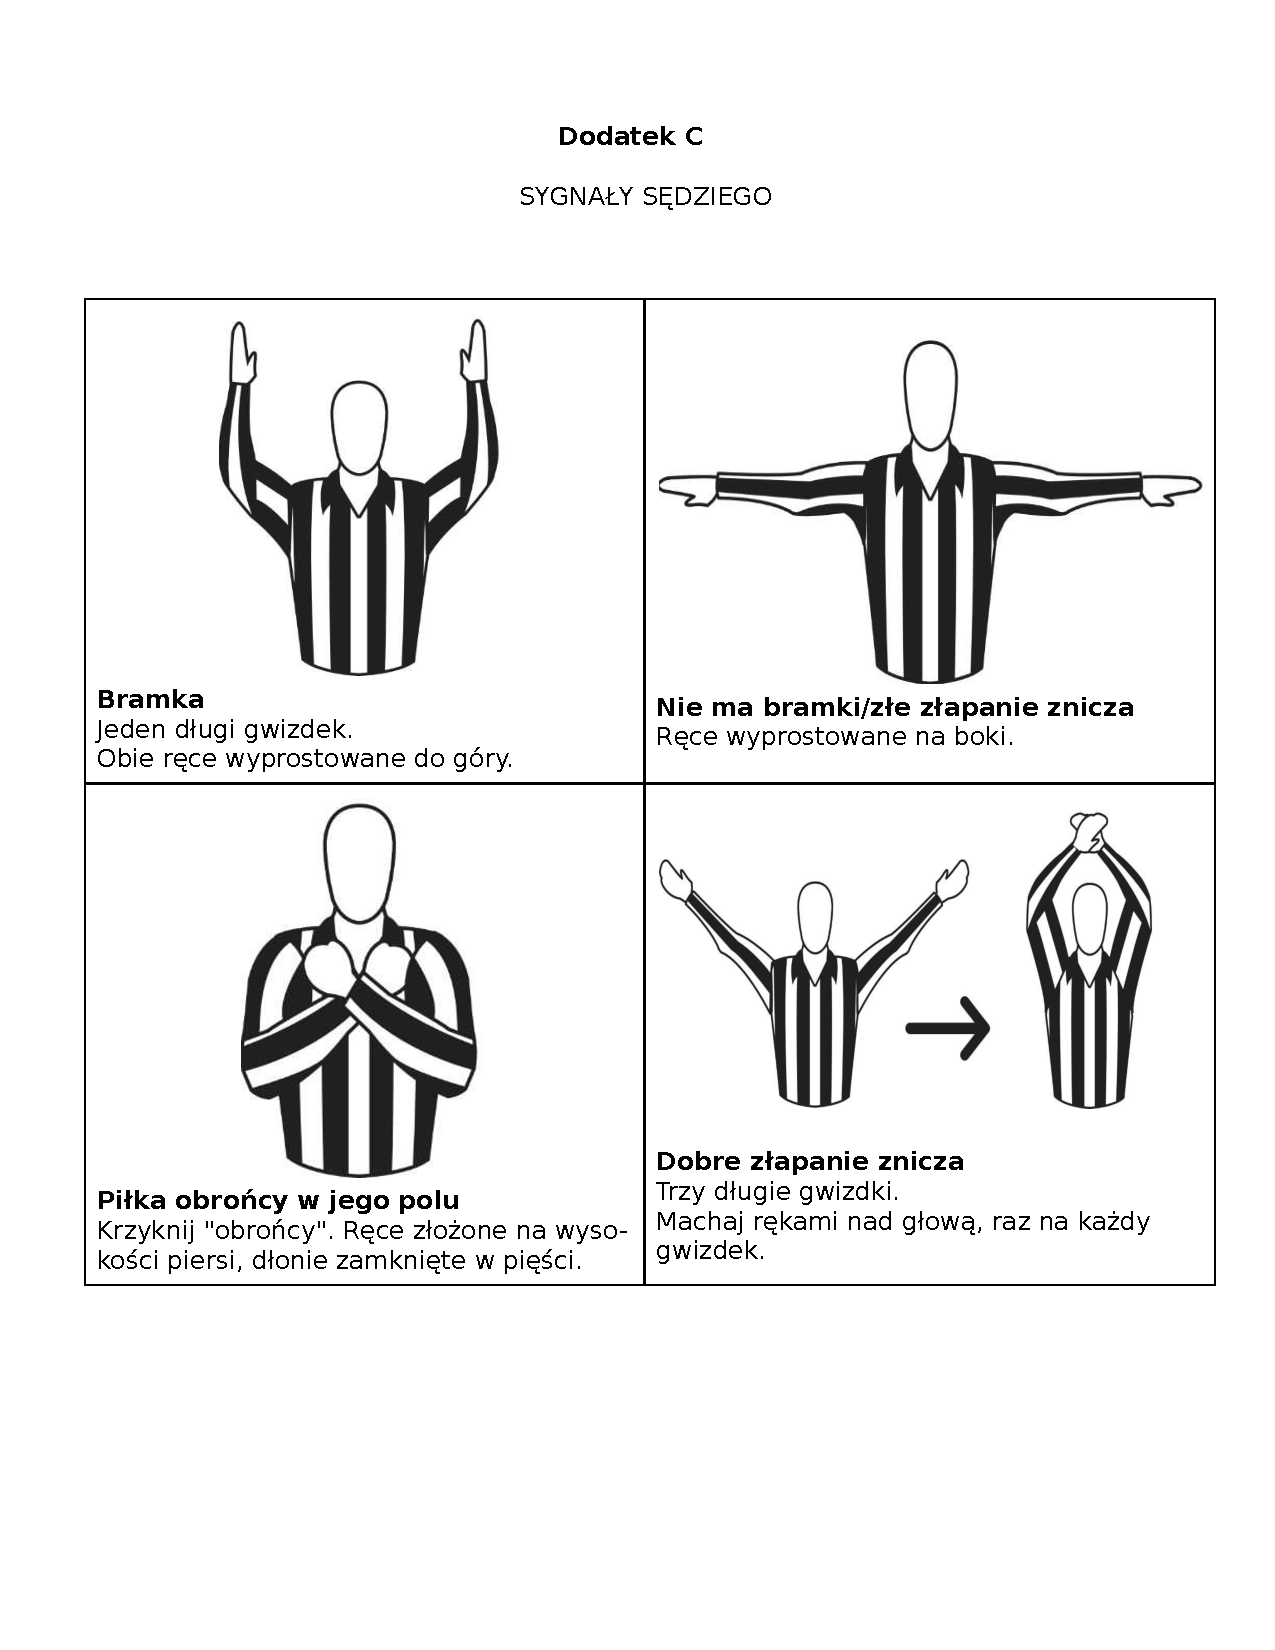
\includepdf[pages={-}]{signals.pdf}

\end{document}
